\clearpage
\appendix
% The appendix carries its own running header, and its tables number A.1, B.1, ...
% so they can be cited unambiguously from the body.
\renewcommand{\headeright}{Appendix}
\counterwithin{table}{section}


\section{GeoScore Component Definitions}
\label{sec:A-geoscore-component-definitions}

GeoScore is a weighted composite of seven validation metrics, each transformed to the unit interval where higher values indicate better performance. Missing components (e.g., holdout metrics when no holdout set is defined) are skipped and the remaining weights are renormalized.

\begin{table}[H]
\centering
\caption{GeoScore components, their weights, and the transformation applied to each raw metric. The weighting reflects the priorities of Section~\ref{sec:geoscore}: ranking quality and spatial equity dominate, while calibration and rare-species performance act as guards against degenerate solutions.}
\label{tab:geoscore-components}
\small
\begin{tabularx}{\linewidth}{lrLLL}
\toprule
Component & Weight & Raw Metric & Transformation & Interpretation \\
\midrule
mAP & 0.20 & Mean average precision across all species & Identity (already in [0, 1]) & Overall species discrimination \\
F1@10\% & 0.20 & F1 score at the 10\% probability threshold & Identity & Calibration-aware classification quality \\
List ratio @10\% & 0.15 & Mean predicted-to-true species count at 10\% threshold & exp($-|$ln(ratio)$|$) & Prediction list length calibration; 1.0 is perfect \\
Watchlist AP & 0.10 & Mean AP over 18 endemic/restricted-range species & Identity & Conservation-relevant discrimination \\
Holdout mAP & 0.10 & mAP on geographically held-out regions & Identity & Spatial generalization \\
Density ratio & 0.20 & mAP(sparse quartile) / mAP(dense quartile) & min(r, 1/r) (peaks at 1.0, penalizes both over- and under-correction) & Spatial equity across observation density \\
pred--density r & 0.05 & Pearson correlation between predicted richness and observer density & 1 $-$ $|$r$|$ (clamped to [0, 1]) & Independence from sampling effort; 0 correlation is ideal \\
\bottomrule
\end{tabularx}
\end{table}


\section{Full Ablation Results Tables}
\label{sec:B-full-ablation-results-tables}

Complete per-run results for all 46 grid-search experiments across Stages A--G. The stage winner is shown in bold in each table. All metrics are computed on the validation set at the best-GeoScore epoch.

\subsection{Stage A --- Loss Family Screening (12 runs)}
\label{sec:B-1-stage-a-loss-family-screening-12-runs}

All runs: model scale 1.0, environmental weight 0.1, no propagation, no habitat head.

\begin{table}[H]
\centering
\caption{Stage A, loss family screening (12 runs). Species ranking is nearly invariant across loss families (mAP 0.536--0.544), but the list ratio spans more than two orders of magnitude (6.2 to 979). Calibration, not ranking, is what separates the candidates, which is why BCE with light label smoothing is carried forward.}
\label{tab:stage-a}
\small
\resizebox{\linewidth}{!}{%
\begin{tabular}{lllrrrrrrrrr}
\toprule
Run & Loss & Setting & GeoScore & mAP & F1@10\% & LR@10\% & Watchlist AP & mAP (sparse) & mAP (dense) & Density Ratio & pred--density r \\
\midrule
A1 (cons) & BCE & smoothing=0.0 & 0.418 & 0.543 & 0.508 & 6.61 & 0.676 & 0.276 & 0.847 & 0.326 & 0.796 \\
\textbf{A1 (default)} & \textbf{BCE} & \textbf{smoothing=0.05} & \textbf{0.422} & \textbf{0.543} & \textbf{0.511} & \textbf{6.43} & \textbf{0.701} & \textbf{0.276} & \textbf{0.847} & \textbf{0.326} & \textbf{0.797} \\
A1 (aggr) & BCE & smoothing=0.10 & 0.420 & 0.543 & 0.515 & 6.22 & 0.671 & 0.276 & 0.847 & 0.326 & 0.799 \\
A2 (cons) & ASL & $\gamma$\_neg=2, clip=0.05 & 0.327 & 0.540 & 0.137 & 48.49 & 0.709 & 0.268 & 0.846 & 0.317 & 0.568 \\
A2 (paper) & ASL & $\gamma$\_neg=4, clip=0.05 & 0.312 & 0.540 & 0.034 & 149.62 & 0.697 & 0.268 & 0.846 & 0.317 & 0.369 \\
A2 (aggr) & ASL & $\gamma$\_neg=6, clip=0.10 & 0.320 & 0.539 & 0.003 & 978.62 & 0.693 & 0.267 & 0.846 & 0.316 & 0.057 \\
A3 (cons) & Focal & $\alpha$=0.50, $\gamma$=1.0 & 0.363 & 0.541 & 0.333 & 17.42 & 0.656 & 0.273 & 0.846 & 0.322 & 0.738 \\
A3 (paper) & Focal & $\alpha$=0.25, $\gamma$=2.0 & 0.347 & 0.540 & 0.259 & 24.77 & 0.665 & 0.273 & 0.846 & 0.323 & 0.702 \\
A3 (aggr) & Focal & $\alpha$=0.75, $\gamma$=4.0 & 0.304 & 0.538 & 0.055 & 102.45 & 0.653 & 0.274 & 0.842 & 0.325 & 0.540 \\
A4 (cons) & AN & $\lambda$=4, neg=1024 & 0.377 & 0.543 & 0.378 & 14.14 & 0.665 & 0.279 & 0.845 & 0.330 & 0.759 \\
A4 (paper) & AN & $\lambda$=8, neg=1024 & 0.367 & 0.542 & 0.319 & 18.86 & 0.706 & 0.280 & 0.844 & 0.332 & 0.736 \\
A4 (aggr) & AN & $\lambda$=16, neg=2048 & 0.350 & 0.536 & 0.260 & 24.76 & 0.689 & 0.275 & 0.840 & 0.328 & 0.703 \\
\bottomrule
\end{tabular}
}
\end{table}

\Needspace*{18\baselineskip}
\subsection{Stage B --- Model Size $\times$ Habitat/Env Transfer (9 runs)}
\label{sec:B-2-stage-b-model-size-habitat-env-transfer-}

Inherited: BCE with label smoothing 0.05.

\begin{table}[H]
\centering
\caption{Stage B, model scale crossed with environmental and habitat transfer (9 runs). GeoScore improves monotonically with scale, while the habitat head fails to help at any size --- the environmental signal is already implicit in species co-occurrence.}
\label{tab:stage-b}
\small
\resizebox{\linewidth}{!}{%
\begin{tabular}{lrlrrrrrrrrr}
\toprule
Run & Scale & Mode & GeoScore & mAP & F1@10\% & LR@10\% & Watchlist AP & mAP (sparse) & mAP (dense) & Density Ratio & pred--density r \\
\midrule
B (s05, coord) & 0.5 & coord\_only & 0.408 & 0.525 & 0.495 & 6.62 & 0.693 & 0.256 & 0.835 & 0.307 & 0.795 \\
B (s05, env) & 0.5 & env\_aux & 0.403 & 0.522 & 0.496 & 6.48 & 0.652 & 0.252 & 0.834 & 0.302 & 0.796 \\
B (s05, hab) & 0.5 & env+habitat & 0.410 & 0.532 & 0.498 & 6.62 & 0.682 & 0.261 & 0.839 & 0.311 & 0.795 \\
B (s10, coord) & 1.0 & coord\_only & 0.420 & 0.540 & 0.510 & 6.34 & 0.696 & 0.272 & 0.845 & 0.321 & 0.794 \\
B (s10, env) & 1.0 & env\_aux & 0.423 & 0.541 & 0.509 & 6.25 & 0.715 & 0.273 & 0.845 & 0.323 & 0.789 \\
B (s10, hab) & 1.0 & env+habitat & 0.419 & 0.546 & 0.507 & 6.62 & 0.676 & 0.280 & 0.849 & 0.330 & 0.792 \\
\textbf{B (s20, coord)} & \textbf{2.0} & \textbf{coord\_only} & \textbf{0.431} & \textbf{0.547} & \textbf{0.519} & \textbf{6.06} & \textbf{0.730} & \textbf{0.282} & \textbf{0.849} & \textbf{0.332} & \textbf{0.795} \\
B (s20, env) & 2.0 & env\_aux & 0.425 & 0.552 & 0.518 & 6.34 & 0.664 & 0.289 & 0.852 & 0.340 & 0.792 \\
B (s20, hab) & 2.0 & env+habitat & 0.424 & 0.550 & 0.512 & 6.60 & 0.685 & 0.286 & 0.850 & 0.336 & 0.787 \\
\bottomrule
\end{tabular}
}
\end{table}

\subsection{Stage C --- Observation Bias Deep Dive (8 runs)}
\label{sec:B-3-stage-c-observation-bias-deep-dive-8-run}

Inherited: BCE default, scale 2.0, coordinate-only.

\begin{table}[H]
\centering
\caption{Stage C, observation bias (8 runs). Label propagation lifts GeoScore from roughly 0.43 to 0.56 at every environmental weight, and raises sparse-quartile mAP from about 0.28 to 0.87. The environmental weight itself is immaterial by comparison.}
\label{tab:stage-c}
\small
\resizebox{\linewidth}{!}{%
\begin{tabular}{lrlrrrrrrrrr}
\toprule
Run & Env Weight & Propagation & GeoScore & mAP & F1@10\% & LR@10\% & Watchlist AP & mAP (sparse) & mAP (dense) & Density Ratio & pred--density r \\
\midrule
C (env=0, off) & 0.0 & off & 0.427 & 0.547 & 0.514 & 6.38 & 0.724 & 0.281 & 0.850 & 0.330 & 0.790 \\
\textbf{C (env=0, on)} & \textbf{0.0} & \textbf{on} & \textbf{0.564} & \textbf{0.694} & \textbf{0.499} & \textbf{4.72} & \textbf{0.638} & \textbf{0.872} & \textbf{0.719} & \textbf{1.212} & \textbf{0.831} \\
C (env=.01, off) & 0.01 & off & 0.430 & 0.554 & 0.524 & 6.05 & 0.676 & 0.293 & 0.852 & 0.344 & 0.794 \\
C (env=.01, on) & 0.01 & on & 0.564 & 0.696 & 0.504 & 4.60 & 0.615 & 0.875 & 0.720 & 1.215 & 0.831 \\
C (env=.1, off) & 0.1 & off & 0.427 & 0.550 & 0.516 & 6.38 & 0.702 & 0.285 & 0.850 & 0.335 & 0.793 \\
C (env=.1, on) & 0.1 & on & 0.561 & 0.689 & 0.502 & 4.62 & 0.604 & 0.868 & 0.717 & 1.210 & 0.833 \\
C (env=.5, off) & 0.5 & off & 0.427 & 0.552 & 0.516 & 6.39 & 0.694 & 0.288 & 0.851 & 0.338 & 0.793 \\
C (env=.5, on) & 0.5 & on & 0.562 & 0.690 & 0.502 & 4.61 & 0.614 & 0.869 & 0.719 & 1.209 & 0.830 \\
\bottomrule
\end{tabular}
}
\end{table}

\subsection{Stage D --- Harmonics Sweep (6 runs)}
\label{sec:B-4-stage-d-harmonics-sweep-6-runs}

Inherited: BCE default, scale 2.0, coordinate-only, no env task, propagation on.

\begin{table}[H]
\centering
\caption{Stage D, harmonics sweep (6 runs). Encoding resolution barely matters: GeoScore varies by 0.004 across all six spatial/weekly harmonic combinations, and the largest setting (eight harmonics each) wins narrowly.}
\label{tab:stage-d}
\small
\resizebox{\linewidth}{!}{%
\begin{tabular}{lrrrrrrrrrrr}
\toprule
Run & Spatial H & Week H & GeoScore & mAP & F1@10\% & LR@10\% & Watchlist AP & mAP (sparse) & mAP (dense) & Density Ratio & pred--density r \\
\midrule
D (ch2, wh4) & 2 & 4 & 0.564 & 0.691 & 0.500 & 4.70 & 0.639 & 0.868 & 0.719 & 1.207 & 0.835 \\
D (ch2, wh8) & 2 & 8 & 0.563 & 0.690 & 0.498 & 4.76 & 0.633 & 0.867 & 0.719 & 1.207 & 0.836 \\
D (ch4, wh4) & 4 & 4 & 0.563 & 0.694 & 0.501 & 4.67 & 0.624 & 0.872 & 0.720 & 1.212 & 0.831 \\
D (ch4, wh8) & 4 & 8 & 0.562 & 0.695 & 0.502 & 4.68 & 0.611 & 0.873 & 0.720 & 1.213 & 0.832 \\
D (ch8, wh4) & 8 & 4 & 0.565 & 0.690 & 0.504 & 4.51 & 0.637 & 0.870 & 0.714 & 1.218 & 0.831 \\
\textbf{D (ch8, wh8)} & \textbf{8} & \textbf{8} & \textbf{0.566} & \textbf{0.698} & \textbf{0.509} & \textbf{4.45} & \textbf{0.612} & \textbf{0.877} & \textbf{0.720} & \textbf{1.219} & \textbf{0.827} \\
\bottomrule
\end{tabular}
}
\end{table}

\Needspace*{16\baselineskip}
\subsection{Stage E --- Augmentation and Yearly Encoding (4 runs)}
\label{sec:B-5-stage-e-augmentation-and-yearly-encoding}

Inherited: full Stage D winner configuration.

\begin{table}[H]
\centering
\caption{Stage E, augmentation and yearly encoding (4 runs). Coordinate jitter yields a marginal gain (0.566 versus 0.565) and yearly encoding none at all; jitter is kept because it costs nothing and slightly improves watchlist AP.}
\label{tab:stage-e}
\small
\resizebox{\linewidth}{!}{%
\begin{tabular}{lccrrrrrrrrr}
\toprule
Run & Jitter & Yearly & GeoScore & mAP & F1@10\% & LR@10\% & Watchlist AP & mAP (sparse) & mAP (dense) & Density Ratio & pred--density r \\
\midrule
E1 (base) & off & off & 0.565 & 0.698 & 0.508 & 4.47 & 0.614 & 0.877 & 0.720 & 1.218 & 0.827 \\
\textbf{E2 (jitter)} & \textbf{on} & \textbf{off} & \textbf{0.566} & \textbf{0.697} & \textbf{0.505} & \textbf{4.55} & \textbf{0.635} & \textbf{0.876} & \textbf{0.719} & \textbf{1.218} & \textbf{0.830} \\
E3 (yearly) & off & on & 0.565 & 0.694 & 0.504 & 4.61 & 0.632 & 0.874 & 0.719 & 1.215 & 0.827 \\
E4 (both) & on & on & 0.565 & 0.695 & 0.507 & 4.55 & 0.615 & 0.873 & 0.718 & 1.215 & 0.826 \\
\bottomrule
\end{tabular}
}
\end{table}

\subsection{Stage F --- Observation Cap Sweep (3 runs + baseline)}
\label{sec:B-6-stage-f-observation-cap-sweep-3-runs-bas}

Inherited: full Stage E winner configuration. Baseline is the E winner (no cap).

\begin{table}[H]
\centering
\caption{Stage F, observation cap sweep (3 runs plus baseline). Capping observations per cell is destructive: at cap 500 the model collapses entirely (mAP 0.002), and even cap 50{,}000 loses a fifth of the uncapped GeoScore and a quarter of its mAP. Frequency-based weighting handles the imbalance better than truncation.}
\label{tab:stage-f}
\small
\resizebox{\linewidth}{!}{%
\begin{tabular}{lrrrrrrrrrr}
\toprule
Run & Cap & GeoScore & mAP & F1@10\% & LR@10\% & Watchlist AP & mAP (sparse) & mAP (dense) & Density Ratio & pred--density r \\
\midrule
\emph{(E winner)} & --- & 0.566 & 0.697 & 0.505 & 4.55 & 0.635 & 0.876 & 0.719 & 1.218 & 0.830 \\
F (cap=500) & 500 & 0.092 & 0.002 & 0.000 & 0.00 & 0.000 & 0.003 & 0.001 & 2.565 & --- \\
\textbf{F (cap=5000)} & \textbf{5000} & \textbf{0.388} & \textbf{0.207} & \textbf{0.169} & \textbf{1.55} & \textbf{0.415} & \textbf{0.344} & \textbf{0.194} & \textbf{1.778} & \textbf{0.531} \\
F (cap=50000) & 50000 & 0.457 & 0.521 & 0.383 & 5.87 & 0.639 & 0.768 & 0.509 & 1.509 & 0.823 \\
\bottomrule
\end{tabular}
}
\end{table}

\emph{Note: cap=5000 is marked as the Stage F "winner" because Stage G (vocabulary scaling) was designed as a diagnostic specifically within the cap=5000 regime --- not because it scores higher than cap=50000. The actual model progression for Stage H carries forward the Stage E winner (no observation cap).}

\subsection{Stage G --- Species Vocabulary Scaling (4 runs + baseline)}
\label{sec:B-7-stage-g-species-vocabulary-scaling-4-run}

Inherited: full Stage F winner configuration. Baseline is the F winner (full vocabulary, \textasciitilde{}11,800 species).

\begin{table}[H]
\centering
\caption{Stage G, species vocabulary scaling (4 runs plus baseline). Absolute scores fall as the vocabulary grows, which is expected --- the task gets harder. The density ratio moves further above 1.0 at the same time, so the sparse quartile is not what the larger vocabularies lose on; all of these runs inherit the Stage F cap, which over-corrects spatial balance in the first place.}
\label{tab:stage-g}
\small
\resizebox{\linewidth}{!}{%
\begin{tabular}{lrrrrrrrrrr}
\toprule
Run & Species & GeoScore & mAP & F1@10\% & LR@10\% & Watchlist AP & mAP (sparse) & mAP (dense) & Density Ratio & pred--density r \\
\midrule
\emph{(F winner)} & 11,827 & 0.388 & 0.207 & 0.169 & 1.55 & 0.415 & 0.344 & 0.194 & 1.778 & 0.531 \\
G (10 spp) & 10 & 0.631 & 0.879 & 0.264 & 0.53 & --- & 0.969 & 0.789 & 1.228 & 0.306 \\
G (100 spp) & 100 & 0.551 & 0.721 & 0.217 & 0.54 & --- & 0.844 & 0.598 & 1.412 & 0.388 \\
G (1000 spp) & 1000 & 0.525 & 0.416 & 0.205 & 1.04 & 0.429 & 0.511 & 0.356 & 1.434 & 0.568 \\
G (5000 spp) & 5000 & 0.434 & 0.262 & 0.187 & 1.45 & 0.532 & 0.388 & 0.240 & 1.613 & 0.594 \\
\bottomrule
\end{tabular}
}
\end{table}

\subsection{Stage H --- Propagation Parameter Optimization (60 Bayesian trials)}
\label{sec:B-8-stage-h-propagation-parameter-optimizati}

Six propagation parameters tuned via TPE sampling with median pruning. Base: Stage E winner. Ecological constraints --- an environmental distance gate and a per-species range cap --- prevent ecologically implausible parameter choices.

The optimization proceeded in two phases. An initial exploratory search of 40 trials ran in three parts: 15 trials over the four unconstrained parameters, which produced the runaway radii discussed in Section~\ref{sec:res-ablation}, followed by 25 trials that added the environmental-distance gate and the per-species range cap. Those 25 used a centroid-based range check, testing each candidate cell against the distance to the species' geographic centroid. This established the importance of tight ecological constraints but was found to penalize migratory species whose breeding and wintering grounds lie far from any centroid. A refined search (20 trials) corrected the distance metric to measure proximity to the nearest original observation of the species, providing a more ecologically appropriate criterion.

\Needspace*{20\baselineskip}
\textbf{Phase 1 --- Exploratory search (40 trials).} Top 10 trials by GeoScore among the 25 that carried the full ecological constraint set; the 15 unconstrained trials are excluded because their GeoScore was computed over a reduced component set and is not comparable:

\begin{table}[H]
\centering
\caption{Stage H, exploratory propagation search: the ten best of the 25 ecologically constrained TPE trials. The sparsity threshold and range cap dominate; $k$ and the environmental distance gate are comparatively free parameters.}
\label{tab:stage-h1}
\small
\begin{tabular}{rrrrrrrr}
\toprule
Trial & GeoScore & $k$ & Radius (km) & Sparsity thresh. & Range spread & Env. dist. gate & Range cap (km) \\
\midrule
\textbf{9} & \textbf{0.637} & \textbf{15} & \textbf{1385} & \textbf{15} & \textbf{2.96} & \textbf{3.29} & \textbf{1071} \\
3 & 0.628 & 19 & 868 & 16 & 2.97 & 2.88 & 1080 \\
1 & 0.625 & 13 & 1317 & 15 & 1.55 & 4.94 & 1126 \\
4 & 0.617 & 10 & 1328 & 16 & 2.38 & 4.44 & 1282 \\
2 & 0.613 & 16 & 906 & 17 & 1.71 & 2.56 & 1590 \\
0 & 0.598 & 10 & 984 & 19 & 1.87 & 2.64 & 1976 \\
5 & 0.580 & 15 & 1151 & 18 & 2.40 & 4.11 & 1462 \\
12 & 0.560 & 20 & 1266 & 6 & 2.43 & 4.06 & 1465 \\
11 & 0.533 & 20 & 1417 & 2 & 2.37 & 4.89 & 1444 \\
13 & 0.523 & 17 & 663 & 7 & 2.53 & 2.47 & 1508 \\
\bottomrule
\end{tabular}
\end{table}

The exploratory search established that the sparsity threshold and range cap are the most sensitive parameters (the top three trials converge on a range cap of 1,071--1,126 km and sparsity threshold of 15--16).

\textbf{Phase 2 --- Refined search with corrected distance metric (20 trials).}

\begin{table}[H]
\centering
\caption{Stage H, refined propagation search with the corrected distance metric: the ten best of 20 TPE trials. With propagation measured from the nearest original observation the optimum moves to a larger range cap (1{,}260--1{,}471\,km across the top three) and a lower sparsity threshold (8--12) than the exploratory search found. Trial 15 is the configuration used in production.}
\label{tab:stage-h2}
\small
\begin{tabular}{rrrrrrrr}
\toprule
Trial & GeoScore & $k$ & Radius (km) & Sparsity thresh. & Range spread & Env. dist. gate & Range cap (km) \\
\midrule
\textbf{15} & \textbf{0.638} & \textbf{20} & \textbf{976} & \textbf{12} & \textbf{0.93} & \textbf{4.99} & \textbf{1471} \\
19 & 0.629 & 17 & 1365 & 8 & 0.54 & 4.26 & 1260 \\
18 & 0.620 & 17 & 1405 & 9 & 1.16 & 4.62 & 1288 \\
14 & 0.620 & 20 & 932 & 15 & 1.12 & 4.90 & 1398 \\
13 & 0.619 & 20 & 959 & 15 & 1.96 & 4.91 & 1406 \\
0 & 0.594 & 15 & 862 & 16 & 2.21 & 2.97 & 443 \\
4 & 0.592 & 9 & 1147 & 4 & 2.55 & 3.90 & 1111 \\
12 & 0.590 & 17 & 1040 & 4 & 2.29 & 3.74 & 889 \\
3 & 0.578 & 8 & 745 & 11 & 2.70 & 3.45 & 713 \\
11 & 0.572 & 16 & 1252 & 11 & 2.26 & 0.66 & 603 \\
\bottomrule
\end{tabular}
\end{table}


\section{Watchlist Species}
\label{sec:C-watchlist-species}

The watchlist comprises 18 endemic or restricted-range species that probe model behavior on geographically constrained distributions. Mean AP is computed per species and averaged to produce the Watchlist AP metric.

\begin{table}[H]
\centering
\caption{The 18 watchlist species: island endemics from three archipelagos plus a few restricted-range taxa.}
\label{tab:watchlist}
\small
\begin{tabular}{lll@{\qquad}lll}
\toprule
Code & Common Name & Region & Code & Common Name & Region \\
\midrule
hawgoo & Hawaiian Goose & Hawaii & riflem1 & Rifleman & New Zealand \\
hawhaw & Hawaiian Hawk & Hawaii & tui1 & Tui & New Zealand \\
elepai & Hawaii Elepaio & Hawaii & kokako3 & North Island Kokako & New Zealand \\
apapan & Apapane & Hawaii & galhaw1 & Galápagos Hawk & Galápagos \\
iiwi & Iiwi & Hawaii & galrai1 & Galápagos Rail & Galápagos \\
hawama & Hawaii Amakihi & Hawaii & galpet & Galápagos Petrel & Galápagos \\
kea1 & Kea & New Zealand & kagu1 & Kagu & New Caledonia \\
nibkiw1 & North Island Brown Kiwi & New Zealand & calcon & California Condor & California \\
takahe3 & South Island Takahe & New Zealand & whocra & Whooping Crane & North America \\
\bottomrule
\end{tabular}
\end{table}


\section{Hyperparameter Search Space}
\label{sec:D-hyperparameter-search-space}

The Bayesian search framework supports 23 tunable parameters. Stage H tunes the six propagation parameters; the full set is available for general hyperparameter optimization.

\begin{table}[H]
\centering
\caption{Hyperparameter search space for the Bayesian optimization framework.}
\label{tab:search-space}
\small
\begin{tabular}{llll}
\toprule
Parameter & Type & Range & Scale \\
\midrule
pos\_lambda & float & [1, 64] & log \\
neg\_samples & categorical & \{128, 256, 512, 1024, 2048, 4096\} & --- \\
label\_smoothing & float & [0.0, 0.1] & linear \\
env\_weight & float & [0.01, 1.0] & log \\
jitter & categorical & \{true, false\} & --- \\
species\_loss & categorical & \{bce, asl, an, focal\} & --- \\
model\_scale & float & [0.25, 3.0] & log \\
coord\_harmonics & int & [2, 8] & linear \\
week\_harmonics & int & [2, 8] & linear \\
asl\_gamma\_neg & float & [1.0, 8.0] & linear \\
asl\_clip & float & [0.0, 0.2] & linear \\
focal\_alpha & float & [0.1, 0.9] & linear \\
focal\_gamma & float & [0.5, 5.0] & linear \\
label\_freq\_weight & categorical & \{true, false\} & --- \\
label\_freq\_weight\_min & float & [0.01, 0.5] & log \\
label\_freq\_weight\_pct\_lo & float & [1.0, 25.0] & linear \\
label\_freq\_weight\_pct\_hi & float & [75.0, 99.0] & linear \\
propagate\_k & int & [1, 20] & linear \\
propagate\_max\_radius & float & [100, 1500] & log \\
propagate\_min\_obs & int & [1, 20] & linear \\
propagate\_max\_spread & float & [0.5, 3.0] & linear \\
propagate\_env\_dist\_max & float & [0.5, 5.0] & linear \\
propagate\_range\_cap & float & [200, 2000] & linear \\
\bottomrule
\end{tabular}
\end{table}


\section{Refuted Design Choices: The Habitat Head}
\label{sec:E-refuted-design-choices}

Hypothesis H3 held that routing predicted environmental features through a secondary species classifier would improve transfer to under-observed regions, by giving the model an explicit habitat pathway rather than relying on coordinates alone. It does not, at any model scale, and the head is absent from the production model. We record its definition and results here because the negative result is informative: it is the strongest evidence that the encoder already internalizes environmental structure from species co-occurrence.

\textbf{Definition.} When enabled, the predicted environmental features are routed through a secondary species head whose logits are combined with those of the direct species head via a learned per-species gate:

\begin{equation*}
g_s = \sigma(W_g \cdot \mathbf{e} + b_g), \qquad
\hat{y}_s = g_s \cdot \hat{y}_s^\text{direct} + (1 - g_s) \cdot \hat{y}_s^\text{habitat}
\end{equation*}

where $\mathbf{e}$ is the encoder embedding and $g_s \in (0, 1)$ is a per-species gate. The gate bias is initialized positive so that the direct head dominates early in training and the habitat pathway contributes only once the environmental predictions become reliable. Environmental features are detached before the habitat head to prevent species-loss gradients from interfering with the regression objective.

The same species loss is applied directly to the habitat head's logits before gating, which gives the habitat pathway an independent learning signal. Without it the head would receive gradients only through a gate initialized to favor the direct head, and the two would deadlock: no gradient to learn from, and no reason for the gate to open.

\textbf{Result.} Across the three scales tested in Stage B (Table~\ref{tab:stage-b}), the habitat configuration never wins: 0.410 versus 0.408 (coordinate-only) at scale 0.5, 0.419 versus 0.420 at scale 1.0, and 0.424 versus 0.431 at scale 2.0. The gap widens with scale, which is consistent with larger models having less need for an explicit habitat pathway. The head adds parameters, a third loss term, and a gating schedule for no measurable return.


\section{Post-Filter Study: Selection and Sampling}
\label{sec:F-post-filter-study-selection-and-sampling}

Supporting detail for the post-filter study of Sections~\ref{sec:protocols} and~\ref{sec:res-filter}.

\subsection{Selection criteria}
\label{sec:F-1-selection-criteria}

Submissions are drawn from the 365 daily app submission logs of 2025 and must satisfy every criterion below. Table~\ref{tab:f-1} gives the yield of each stage.

\begin{enumerate}
  \item \textbf{Confident on-device detection} --- the submission's primary detection score exceeds
0.5.
  \item \textbf{No human vocalization} --- the class \texttt{Human} appears nowhere in the ten detections
reported per submission, which removes recordings dominated by speech.
  \item \textbf{Duration 2.5--3.5 s} --- a single centered 3 s window then covers essentially the whole
recording, so classifier scores are comparable across files and no segment-aggregation rule has to be chosen.
  \item \textbf{Valid coordinates} --- finite, |lat| $\leq$ 90, |lon| $\leq$ 180, and not (0, 0).
  \item \textbf{Valid date and week} --- the timestamp parses, falls in 2025, matches the date of the
log it came from, and the week field is a real week number rather than an "unknown week" sentinel.
\end{enumerate}


\begin{table}[H]
\centering
\caption{Candidate pool after each selection stage (2025, all 365 days).}
\label{tab:f-1}
\small
\begin{tabular}{lrr}
\toprule
Stage & Submissions & Retained \\
\midrule
All submissions & 39,567,545 & 100.0\% \\
Primary score > 0.5 & 17,498,115 & 44.2\% \\
No human vocalization & 14,534,453 & 36.7\% \\
Duration 2.5--3.5 s & 1,835,497 & 4.6\% \\
Valid coordinates & 1,835,497 & 4.6\% \\
Valid date and week & \textbf{1,718,002} & \textbf{4.3\%} \\
\bottomrule
\end{tabular}
\end{table}

The app records its week index with a different 48-week convention than the geomodel (0-based, with month-bucket boundaries at days 7, 15 and 24, against the geomodel's 1-based boundaries at days 7, 14 and 21). The geomodel week is therefore recomputed from the recording timestamp; the recorded week field is used only as a validity check.

\subsection{Balanced sampling}
\label{sec:F-2-balanced-sampling}

Candidates are assigned to H3 resolution-2 cells (\textasciitilde{}86,000 km$^2$; 1,216 cells occupied) and drawn by a two-level round robin: cells are visited in a fixed random order, one recording is taken per visit, and within a cell the draw rotates over \texttt{deviceId} so that no single device dominates its cell. Cells that run out of candidates drop out, which redistributes their unused quota over the remaining cells until the target count is reached. The result is an equal per-cell quota wherever the pool allows one (per-cell count: min 1, median 21, max 304).


\begin{table}[H]
\centering
\caption{Regional composition before and after balancing (approximate bounding boxes).}
\label{tab:f-2}
\small
\begin{tabular}{lrr}
\toprule
Region & Candidate pool (1,718,002) & Study set (100,032) \\
\midrule
Europe & 83.7\% & 39.0\% \\
North America & 5.8\% & 27.7\% \\
Asia & 1.3\% & 16.3\% \\
South America & 0.5\% & 6.7\% \\
Africa & 8.3\% & 5.2\% \\
Oceania & 0.5\% & 4.5\% \\
Other & 0.0\% & 0.7\% \\
\bottomrule
\end{tabular}
\end{table}

Europe still leads because H3 cells are equal-area units and Europe simply occupies more of them than Oceania does, but its share falls by a factor of 2.1 while the four under-represented regions gain roughly five- to fourteen-fold.

\begin{figure}[H]
\centering
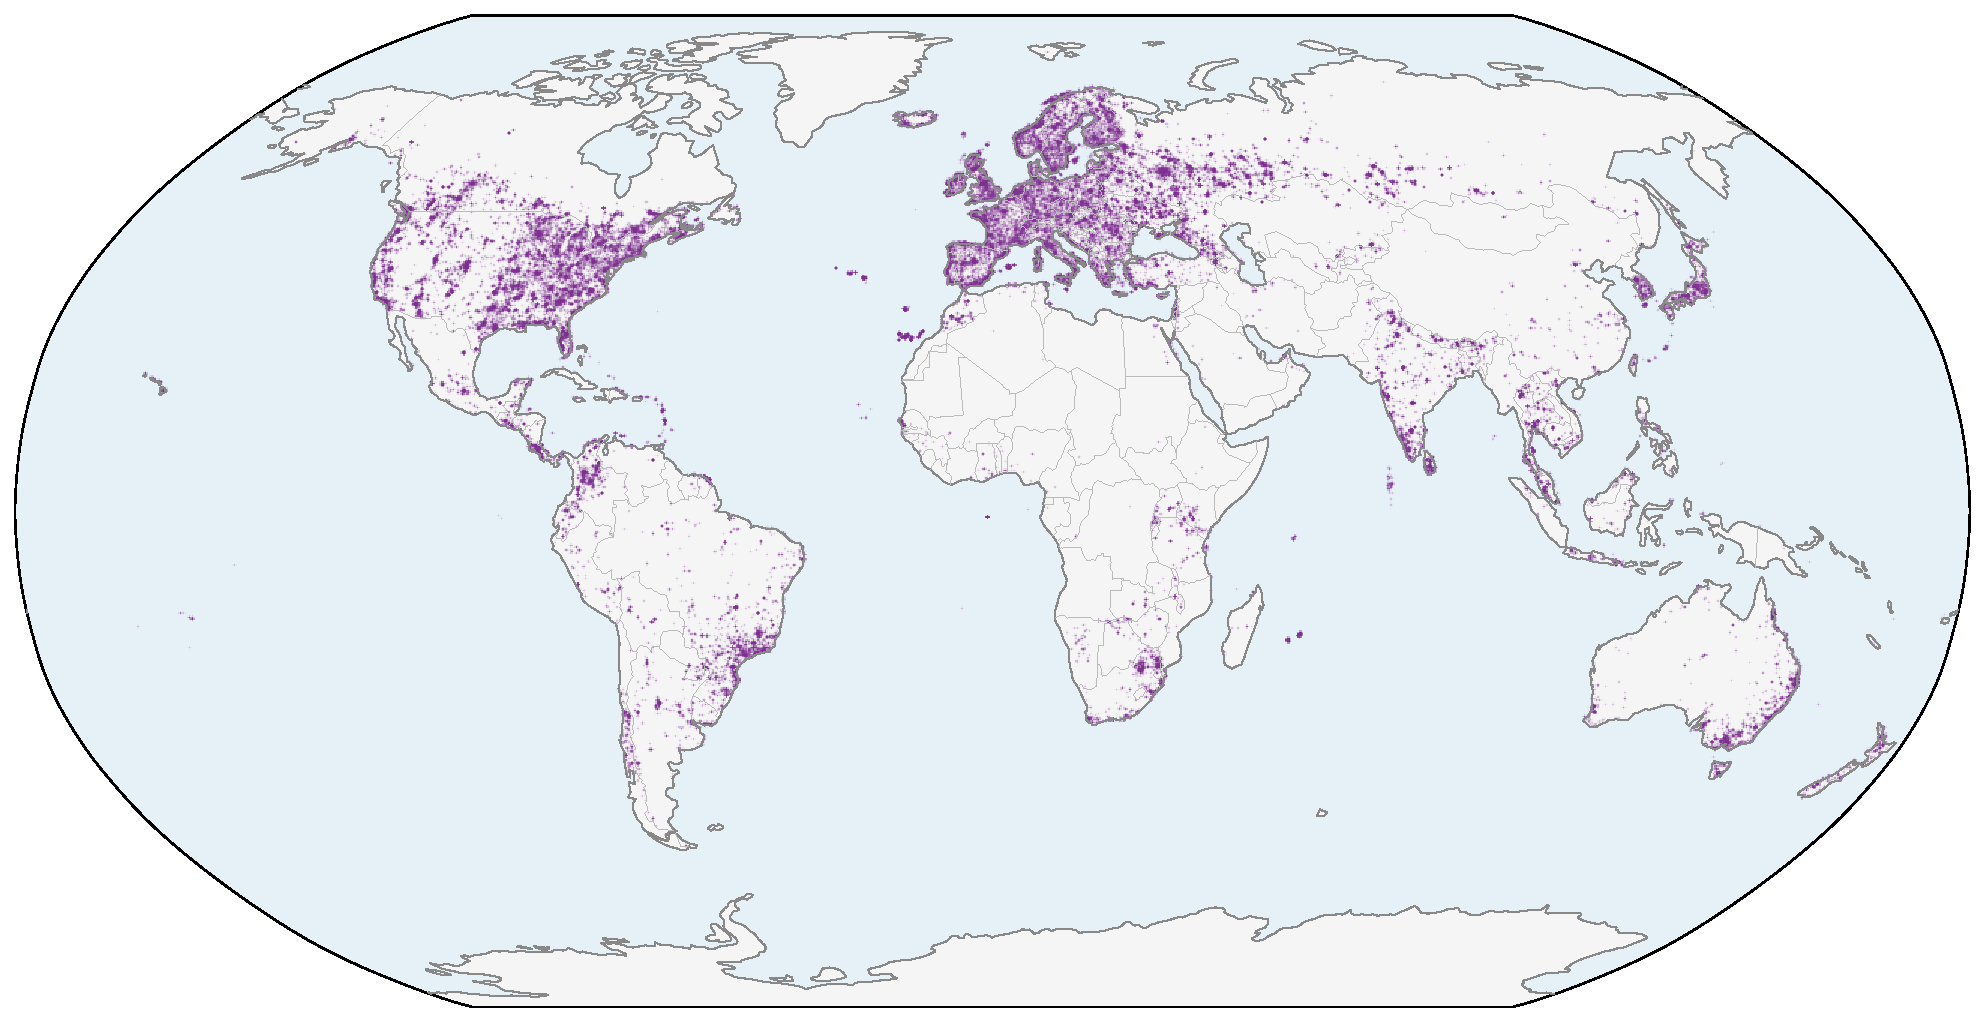
\includegraphics[width=\linewidth]{figures/filter_study_sample_map.pdf}
\caption{The study set: 100,032 BirdNET app submissions from 2025, drawn with an equal quota per occupied H3 resolution-2 cell. What remains visible is the residual density within regions, since the quota equalises cells rather than area.}
\label{fig:sample-map}
\end{figure}

\subsection{Classification}
\label{sec:F-3-classification}

Each recording's centered 3 s window is decoded to mono and resampled to 32 kHz, the rate the classifier expects, then passed through the BirdNET+ V3.0 developer preview (\texttt{V3.0-preview3.1\_Global\_11K}; \citealp{lasseck2026birdnetv3}). All 100,032 selected files decoded successfully. Class matching between the classifier's 11,560 labels and the geomodel's 12,012 species is by scientific name and covers 10,333 classifier classes (89.4\%); on the study set this leaves 99.37\% of top-3 bird predictions with a geomodel counterpart. The 0.63\% without one are excluded from the analysis rather than counted as rejections, and are predominantly recent taxonomic splits.


\begin{table}[H]
\centering
\caption{Rejection rate by region at $t = 0.15$ (see Sections~\ref{sec:res-filter} and~\ref{sec:disc-practice}).}
\label{tab:f-3}
\small
\begin{tabular}{lrrr}
\toprule
Region & Recordings & Bird predictions & Rejection rate \\
\midrule
North America & 27,717 & 82,291 & 11.2\% \\
Europe & 38,958 & 115,780 & 14.5\% \\
South America & 6,684 & 19,915 & 22.8\% \\
Oceania & 4,543 & 13,350 & 23.6\% \\
Asia & 16,257 & 48,037 & 34.6\% \\
Africa & 5,205 & 14,948 & 46.4\% \\
Other & 651 & 1,930 & 55.6\% \\
\bottomrule
\end{tabular}
\end{table}


\Needspace*{34\baselineskip}
\section{Data Pipeline}
\label{sec:G-data-pipeline-diagram}

Figure~\ref{fig:pipeline} summarizes the sequence described in Section~\ref{sec:data}.

\begin{figure}[H]
\centering
\begin{tikzpicture}[
  font=\small,
  node distance=7mm and 10mm,
  box/.style={draw, rounded corners=2pt, align=center, inner sep=3pt,
              minimum height=7mm, fill=gray!5},
  src/.style={box, fill=blue!8},
  data/.style={box, fill=orange!12},
  outbox/.style={box, fill=green!10},
  ->, >=latex, thick,
]
% --- sources ---
\node[src] (gbif) {GBIF Darwin Core Archive\\(eBird, iNaturalist, observation.org)};
\node[src, right=of gbif] (gee) {Google Earth Engine};

% --- per-source processing ---
\node[box, below=of gbif] (filter) {Filter and clean\\(taxonomy, coordinates, dates)};
\node[box, below=of gee] (h3env) {H3 grid +\\environmental sampling};

\node[box, below=of $(filter)!0.5!(h3env)$] (combine) {Merge into H3 cells};
\node[data, below=of combine] (parquet) {Parquet dataset:\\H3 cells $\times$ 48 weeks\\$\times$ species lists + env.\ features};
\node[box, below=of parquet] (flatten) {Flatten to samples\\(lat, lon, week, species, env.)};
\node[box, below=of flatten] (prop) {Label propagation\\(env.-space $k$-NN)};
\node[box, below=of prop] (pre) {Normalize, encode,\\location-based split};

% --- outputs ---
\node[outbox, below left=9mm and 8mm of pre] (train) {Training set};
\node[outbox, below=9mm of pre] (val) {Validation set};
\node[outbox, below right=9mm and 8mm of pre] (hold) {Holdout regions\\(optional)};

\draw (gbif) -- (filter);
\draw (gee) -- (h3env);
\draw (filter) -- (combine);
\draw (h3env) -- (combine);
\draw (combine) -- (parquet);
\draw (parquet) -- (flatten);
\draw (flatten) -- (prop);
\draw (prop) -- (pre);
\draw (pre) -- (train);
\draw (pre) -- (val);
\draw (pre) -- (hold);
\end{tikzpicture}
\caption{Data pipeline. Occurrence records from the GBIF Darwin Core Archive and
environmental layers from Google Earth Engine are merged into H3 cells, expanded to
weekly samples, and augmented by label propagation in environmental space before the
location-based train/validation/holdout split.}
\label{fig:pipeline}
\end{figure}


\Needspace*{24\baselineskip}
\section{eBird Status and Trends: Full Results}
\label{sec:H-ebirdst-full-results}

Per-species metrics and additional range overlap maps supporting Section~\ref{sec:res-ebirdst}.

\begin{table}[H]
\centering
\caption{Range overlap with eBird Status and Trends on a 0.5\textdegree{} grid at threshold 0.15 (production model, scale 0.75). Recall exceeds precision in 15 of 20 comparisons, which is the model over-predicting at range margins rather than missing core range. AUC, which needs no threshold, stays above 0.94 everywhere except Northern Wheatear in July.}
\label{tab:ebirdst}
\footnotesize
\begin{tabular}{l rrrrr rrrrr}
\toprule
& \multicolumn{5}{c}{Week 1 (January)} & \multicolumn{5}{c}{Week 26 (July)} \\
\cmidrule(lr){2-6}\cmidrule(l){7-11}
Species & Jacc. & Prec. & Rec. & F1 & AUC & Jacc. & Prec. & Rec. & F1 & AUC \\
\midrule
Amur Falcon & 0.709 & 0.727 & 0.966 & 0.830 & 0.994 & 0.648 & 0.870 & 0.718 & 0.787 & 0.992 \\
Blue-and-yellow Macaw & 0.690 & 0.705 & 0.970 & 0.817 & 0.974 & 0.720 & 0.741 & 0.963 & 0.837 & 0.974 \\
Bobolink & 0.767 & 0.885 & 0.852 & 0.868 & 1.000 & 0.591 & 0.619 & 0.928 & 0.743 & 0.972 \\
Common Swift & 0.764 & 0.930 & 0.811 & 0.866 & 0.993 & 0.767 & 0.783 & 0.975 & 0.868 & 0.943 \\
European Bee-eater & 0.795 & 0.908 & 0.865 & 0.886 & 0.988 & 0.772 & 0.804 & 0.951 & 0.871 & 0.981 \\
Northern Cardinal & 0.590 & 0.596 & 0.983 & 0.742 & 0.974 & 0.684 & 0.696 & 0.976 & 0.812 & 0.989 \\
Northern Wheatear & 0.483 & 0.667 & 0.636 & 0.651 & 0.979 & 0.657 & 0.685 & 0.942 & 0.793 & 0.880 \\
Ruby-throated Hummingbird & 0.407 & 0.414 & 0.959 & 0.578 & 0.988 & 0.651 & 0.654 & 0.993 & 0.789 & 0.983 \\
Rufous Hummingbird & 0.199 & 0.210 & 0.787 & 0.331 & 0.964 & 0.570 & 0.571 & 0.998 & 0.726 & 0.979 \\
Wilson's Warbler & 0.522 & 0.538 & 0.944 & 0.686 & 0.989 & 0.651 & 0.659 & 0.982 & 0.789 & 0.968 \\
\midrule
\textbf{Mean (20 pairs)} & \multicolumn{10}{c}{Jaccard \textbf{0.632} \quad Precision \textbf{0.683} \quad Recall \textbf{0.910} \quad F1 \textbf{0.764} \quad AUC \textbf{0.975}} \\
\bottomrule
\end{tabular}
\end{table}

Figure~\ref{fig:rangemaps} in Section~\ref{sec:res-ebirdst} shows three long-distance migrants; Figure~\ref{fig:rangemaps-residents} below shows two residents and one medium-distance migrant at the same two weeks. The remaining four comparison species follow the same patterns and are omitted for space. Colors are as in Figure~\ref{fig:rangemaps}: purple marks cells the geomodel predicts but S\&T does not, green marks cells S\&T reports but the geomodel misses, yellow marks agreement.

\begin{figure}[H]
\centering
\begin{subfigure}[t]{0.30\linewidth}
  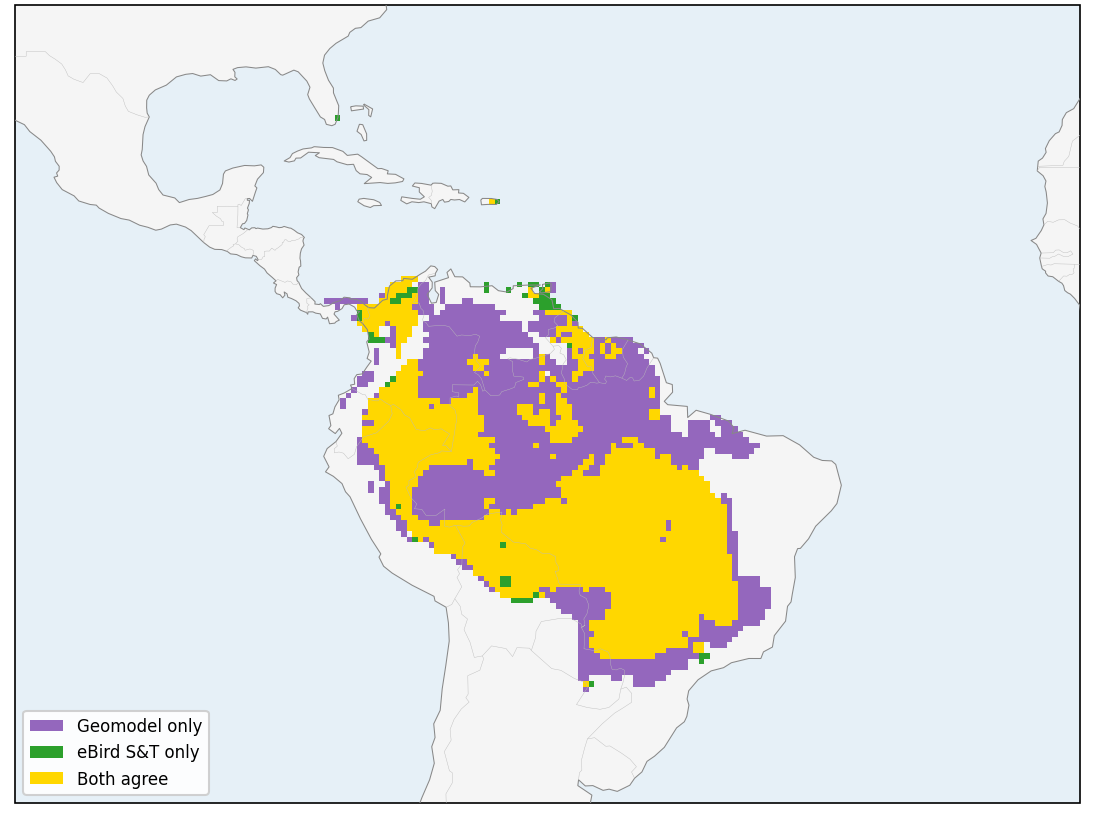
\includegraphics[width=\linewidth]{figures/ebirdst_baymac_week1.png}
  \caption{Blue-and-yellow Macaw, week 1}
\end{subfigure}
\hfill
\begin{subfigure}[t]{0.30\linewidth}
  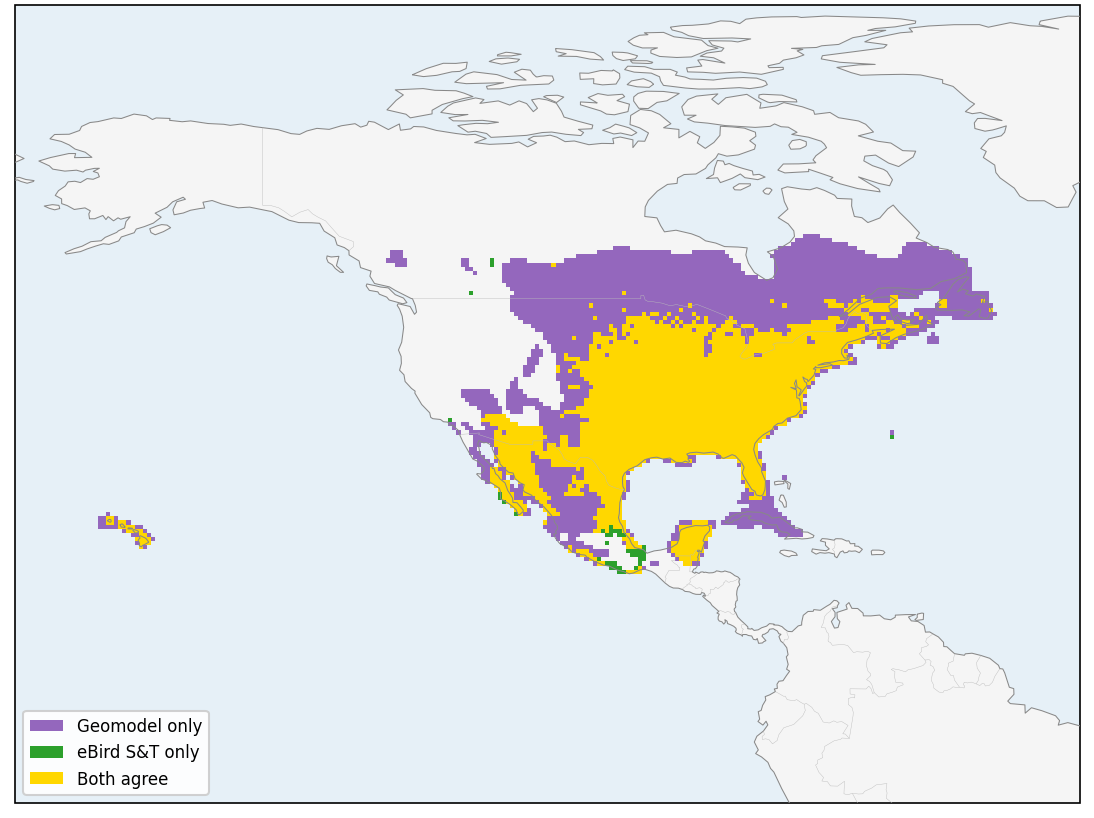
\includegraphics[width=\linewidth]{figures/ebirdst_norcar_week1.png}
  \caption{Northern Cardinal, week 1}
\end{subfigure}
\hfill
\begin{subfigure}[t]{0.30\linewidth}
  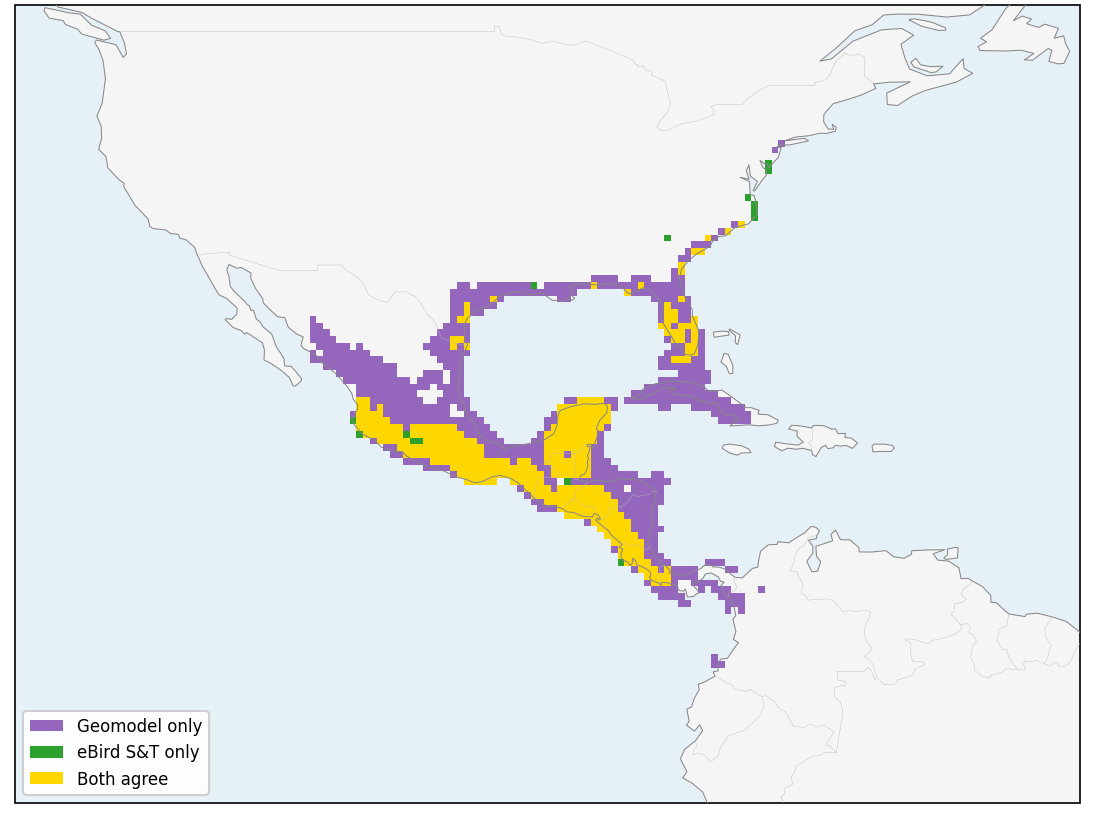
\includegraphics[width=\linewidth]{figures/ebirdst_rthhum_week1.png}
  \caption{Ruby-throated Hummingbird, week 1}
\end{subfigure}

\vspace{6pt}

\begin{subfigure}[t]{0.30\linewidth}
  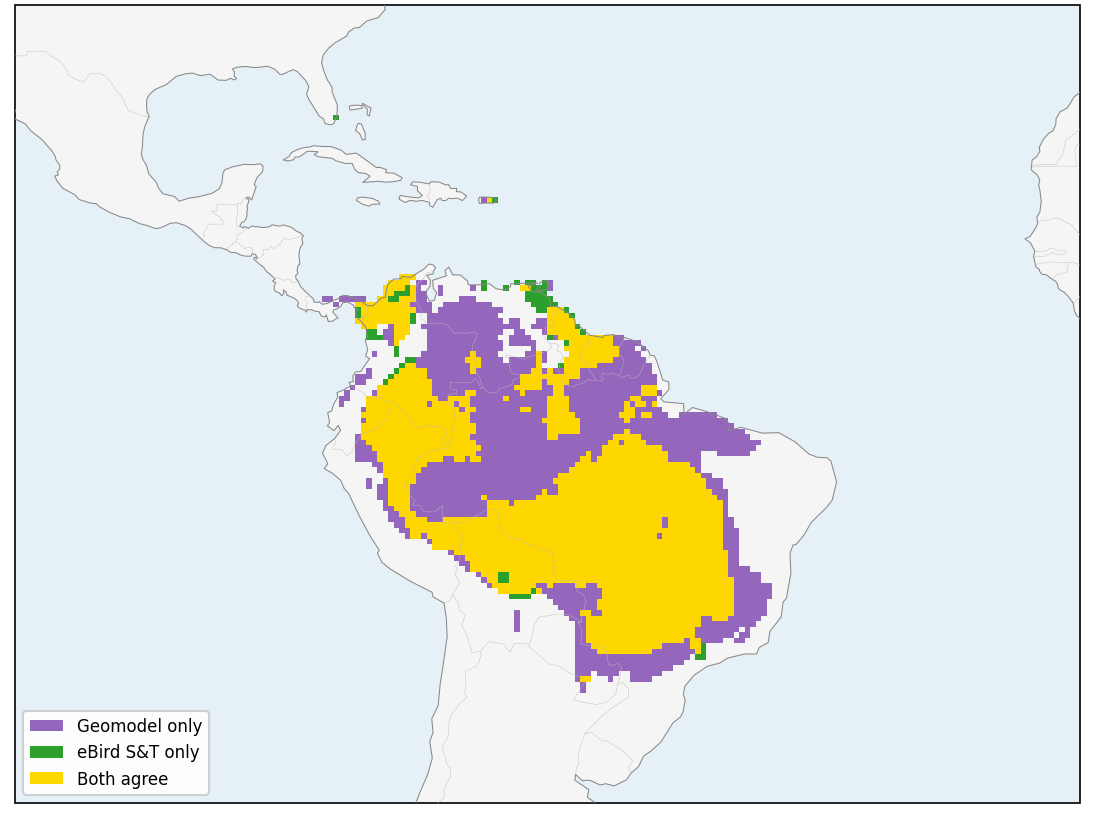
\includegraphics[width=\linewidth]{figures/ebirdst_baymac_week26.png}
  \caption{Blue-and-yellow Macaw, week 26}
\end{subfigure}
\hfill
\begin{subfigure}[t]{0.30\linewidth}
  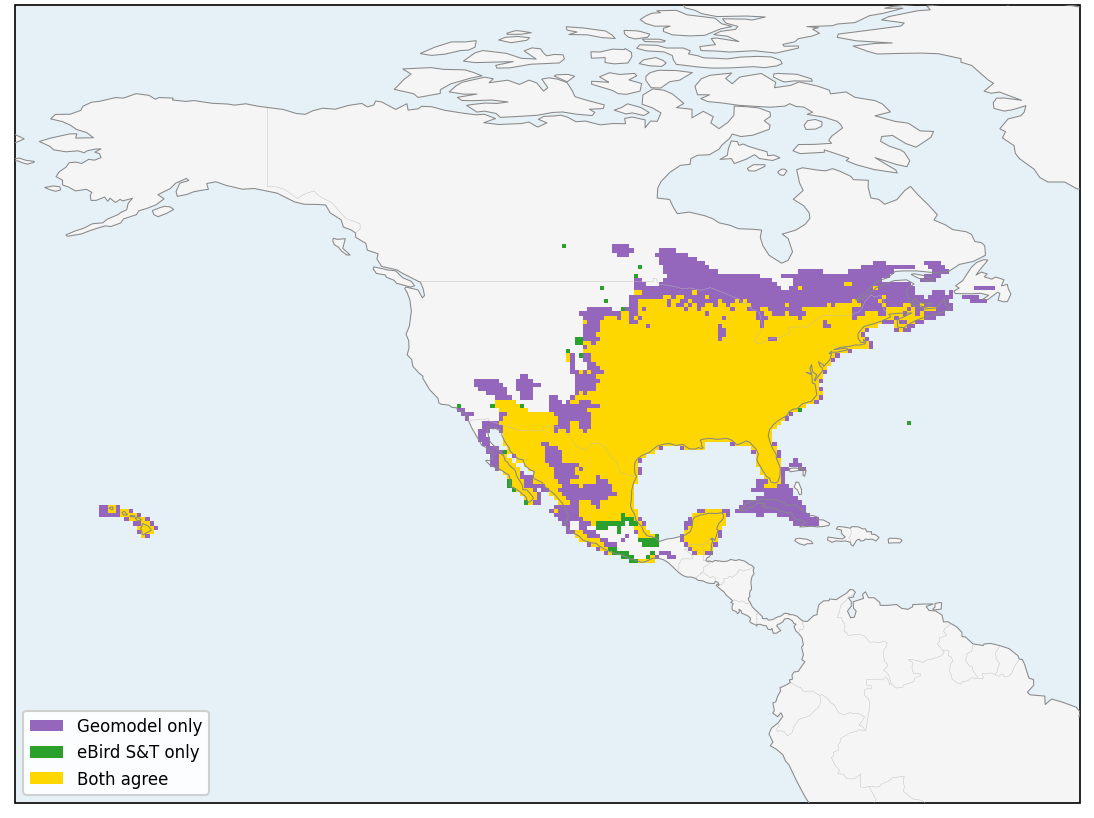
\includegraphics[width=\linewidth]{figures/ebirdst_norcar_week26.png}
  \caption{Northern Cardinal, week 26}
\end{subfigure}
\hfill
\begin{subfigure}[t]{0.30\linewidth}
  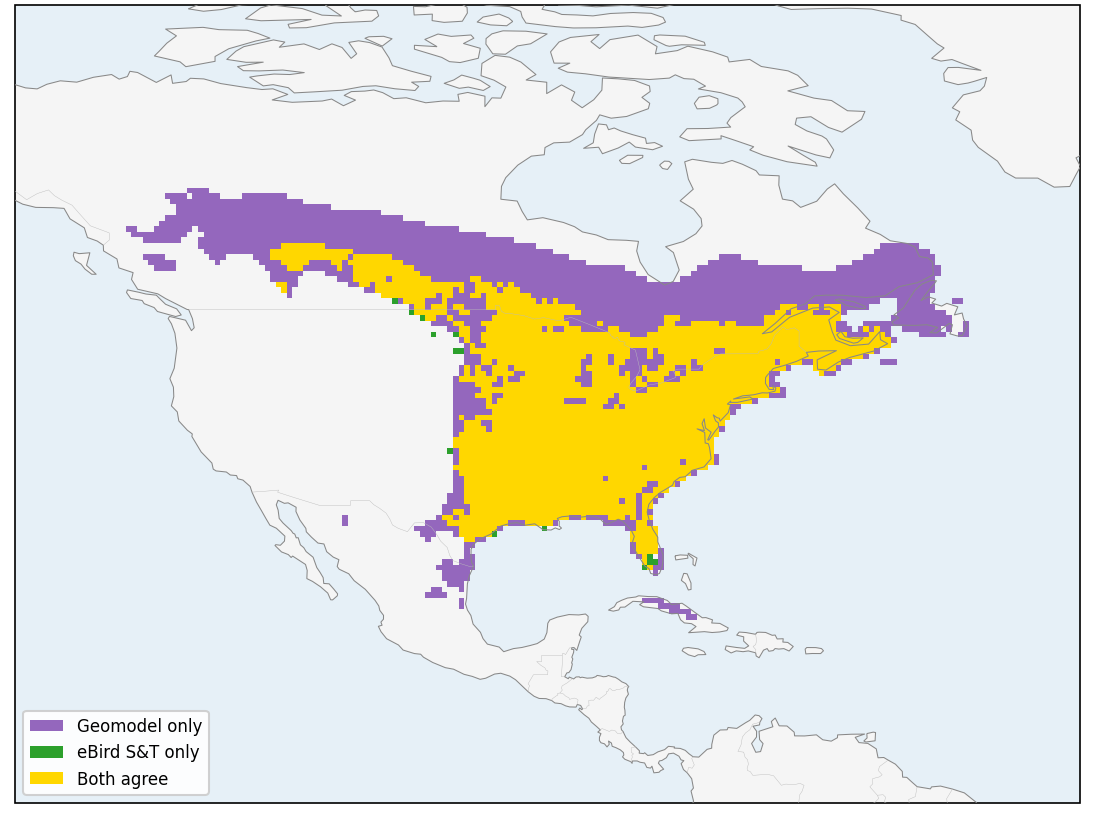
\includegraphics[width=\linewidth]{figures/ebirdst_rthhum_week26.png}
  \caption{Ruby-throated Hummingbird, week 26}
\end{subfigure}
\caption{Range overlap for two residents and one medium-distance migrant, January (top) and July
(bottom). The residents are nearly identical across seasons (Jaccard 0.690 versus 0.720 and 0.590
versus 0.684), so weekly conditioning invents no spurious seasonality. Ruby-throated Hummingbird
shows the study's typical winter failure mode: the January panel over-predicts across Central
America, where S\&T concentrates the species into a narrower wintering band.}
\label{fig:rangemaps-residents}
\end{figure}

